\documentclass{article}
\usepackage[utf8]{inputenc}
\usepackage{biblatex}
\usepackage{graphicx}
\usepackage[font=small, labelfont=bf]{caption}
\usepackage{amsmath}
\usepackage{amsthm}
\usepackage{amsfonts}
\usepackage{mathabx}
\usepackage{tikz}
\usepackage{esvect}
\usepackage{changepage}
\usetikzlibrary{automata, positioning, arrows}

\title{Computability, its Proof by Construction, and the Halting Problem}
\author{Oluwafunke Alliyu, Ethan Balcik, Paul John Balderston, Sen Zhu}
\date{April 2021}

\begin{document}
\theoremstyle{definition}
\newtheorem{exmp}{Example}[section]
\newtheorem{defin}{Definition}[section]
\newtheorem{prf}{Proof}[section]

\maketitle

\section{Introduction}
Our world’s infastructure is entirely reliant upon digital computers. Despite
their ubiquity, the high levels of abstraction at which such devices are typically
used leads the majority of users to have little to knowledge of their underlying
functionalitiy. It is in the spirit of elucidating the working of computational
devices that we discuss the most essential topic in the theory of computation, the
computatability of functions. We begin by providing a list of requisite definitions
nessacry to define and describe mechanisms by which one may determine if a
function is computable. We introduce the reader to the Turing Machine, a
conceptual model of an all purpose computer. Once familiarzing the reader
with the aforementioned concepts we invoke the use of a Turing Machine to
rigorously prove of the computability of an even weight verification function for
a binary input string. We conclude with a discussion of the Halting Problem in
order to further extend our discussion to noncomputable functions. \cite{1}

\section{Background}
It is essential to understanding the following definitions of elementary set theory prior to the discussion of Turing machines and their functionality.
\begin{defin}
A \textbf{set} is a well-defined collection of objects. The objects which a set is composed of are referred to as its \textbf{elements} or \textbf{members}.
\begin{itemize}
\item $a \in S$ represents that a is 'in' $S$, or that a is a elements of $S$
\item $a \notin S$ represents that a is not an element of $S$
\item $\emptyset$ represents an empty set
\end{itemize}
\end{defin}
\begin{defin}
Consider the sets $X$ and $Y$ with $y \in Y$ and $x \in X$ where $y$ and $x$ are arbitary elements. If every element $y \in Y$ is such that $y \in X$, then $Y$ is a \textbf{subset} of $X$, which may be written as $Y\subseteq X$.
If $Y$ is a subset of $X$, but there exsists at least one $x \in X$ for which $x \notin Y$ then $Y$ is a \textbf{proper subset} of X, which we write as $Y \subset X$.
\begin{itemize}
\item Any set $X$ contains the subsets $X \subseteq X$ and $\emptyset \subseteq X$, which are distinct unless X is empty.
\end{itemize}
\end{defin}
\begin{defin}
The \textbf{Cartesian product} $X \times Y \coloneq \{ (x, y): x \in X$ and $y \in Y \}$, is defined to be the set of all ordered pairs such that $x \in X$ and $y \in Y$.
\begin{itemize}
\item The Cartesian product of $n$ sets, where $n \in \mathbb{N}$, is given as
$X_{1}\times X_{2} \times {...} \times X_{n} \coloneq \{( x_{1},x_{2},{...},x_{n}):x_{i}\in X_{i}$ for each $i = 1,2,{...},n\}$
\item For a given set $X$ and some aribitrary $n \in \mathbb{Z}_{\geq 0}$, the nth \textbf{Cartesian power} of $X$ is defined by
$X^{n} \coloneq X \times {...} \times X = \{(x_{1},{...},x_n) ; x_{1},x_{2},{...},x_{n}\in X\}$, and it is the cartesian product of $X$ with itself taken $n$ times.
\end{itemize}
\end{defin}
\begin{defin}
A \textbf{function} $f \subseteq X \times Y$, such that each $x \in X$ is mapped to exactly one $y \in Y$, forming the 2-tuple (or ordered pair) $(x, y) \in f$
\end{defin}

\section{Turing Machines}
The Turing Machine is a general-purpose computing device capable of performing any given algorithmic computation.\cite{2}.  While the model itself is an abstraction, any instantion of a Turing Machine, physical or platonic, is comprised of the following:
\begin{itemize}
	\item A "control box" which stores a program of finite size, formally known as the \textbf{transition function}.
	\item A tape with a potentially infinite number of memory spaces in which symbols can be stored, read, and written into each indivdua spacel.
	\item A read-write mechanism which the tape is fed through. \cite{3}
\end{itemize}
\begin{figure}[h]
	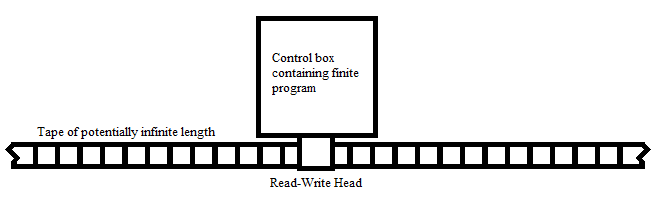
\includegraphics[width=0.85\textwidth]{figure-3-1}
	\centering
	\setlength{\belowcaptionskip}{-10pt}
	\caption{A simple visualization of a Turing machine.  Note that spaces along the tape would be filled with symbols which can be read and written using the read-write head on the machine.}
\end{figure}

\noindent Prior to presenting the formal definiton of a Turing Machine we must introduce the following items.

\begin{defin}
	An \textbf{alphabet} is a finite set of arbitrary characters which can be used in some code or language.
\end{defin}
\noindent For example, the english alphabet (ignoring all punctuation and special characters) may define its alphabet as $A_{english} \coloneq \{ a, b, ... , z \}$
\begin{defin}
	A \textbf{word} $\vv{x}$ is a string of characters, each of which belonging to some alphabet $A$.
\end{defin}
\noindent Following from the previous example, we may construct words of varying lengths using the english alphabet, such as "the", "dog", "was", and "running".  Each character composing each of these words belong to the alphabet $A_{english}$ defined above.
\begin{defin}
	A \textbf{language} $L$ is the set of all possible words $\vv{x} \in L$ of varying length, over some alphabet $A$.
\end{defin}

\noindent Any combination of english characters imaginable will certainly be a member of the language $L_{english}$ which is defined on the alphabet $A_{english}$.\\

\noindent Having introduced the items above we may now develope a formal definiton of the Turing Machine.

\begin{defin}
	A \textbf{Turing Machine} is a 7-Tuple, $(Q, \Sigma, \Gamma, \delta, q_{0}, q_{accept}, q_{reject})$, where:
\end{defin}
\begin{itemize}
	\item $Q$ is a finite set containing the states of the machine
	\item $\Sigma$ is a finite set containing the machine's \textbf{input alphabet}
	\item $\Gamma$ is the finite set containing th emachine's \textbf{tape alphabet} such that the \textbf{blank symbol} $\textvisiblespace \in \Gamma$ and $\Sigma \subseteq \Gamma$
	\item $\delta$ is the \textbf{transition function} $\delta: Q \times \Gamma \to Q \times \Gamma \times \{L, R\}$
	\item $q_{0}$ is the \textbf{starting state} $q_{0} \in Q$
	\item $q_{accept}$ is the \textbf{accept state} $q_{accept} \in Q$
	\item $q_{reject}$ is the \textbf{reject state} $q_{reject} \in Q$ such that $q_{reject} \neq q_{accept}$ \cite{2}
\end{itemize}
\begin{defin}
	A \textbf{configuration} is a string of characters representing the position of a Turing machine's read-write head along its tape, as well as the characters on the tape.  It is written as a string of the tape's characters listed starting from the left-most character and working right, with the state $q_{n} \in Q$ inserted to the left of the character currently being read by the read-write head of the machine.
\end{defin}
\begin{defin}
	A \textbf{computation} is a sequence of configurations which represents the sequence of transition function operations run by a Turing machine given some input. \cite{6}
\end{defin}
\noindent To exemplify these definitions, we provide an instantiation of a Turing Machine with a specific input, and an algorthim, running on the input.
\begin{exmp}
Let's imagine a Turing machine running an algorithm which decides whether a binary string of length $n : n \in \mathbb{Z}_{\geq 0}$ has an even weight, such that number of 1s in the binary string is even.  Our Turing Machine will execute the following algorithm:
\begin{enumerate}
	\item Read the first bit of the string
	\item If the first bit of the string is a '0', transition to state $q_{3}$.
	\item If the first bit of the string is a '1', transition to state $q_{2}$.
	\item While in states $q_{2}$ and $q_{3}$, transition to the other state if a '1' is read, remain in current state if '0' is read.
	\item If in state $q_{2}$ and reading '$\textvisiblespace$' character, terminate in state $q_{reject}$
	\item If in state $q_{3}$ and reading '$\textvisiblespace$' charactre, terminate in state $q_{accept}$.
\end{enumerate}
\noindent This particular Turing machine may be given formally as \\

\centerline{$M \coloneq (Q, \Sigma, \Gamma, \delta, q_{1}, q_{accept}, q_{reject})$}

\noindent such that:
\begin{itemize}
	\item $Q \coloneq \{ q_{1}, q_{2}, q_{3}, q_{accept}, q_{reject} \}$
	\item $\Sigma \coloneq \{ 0, 1 \}$
	\item $\Gamma \coloneq \{ 0, 1, \textvisiblespace \}$
	\item The transition function $\delta$ is given as the following instruction set
\end{itemize}
\begin{center}
	\begin{tabular}{ c }
	$\delta(q_{1}, 0) = (q_{3}, 0, R)$ \\
	$\delta(q_{1}, 1) = (q_{2}, 1, R)$ \\
	$\delta(q_{1}, \textvisiblespace) = (q_{3}, \textvisiblespace, R)$ \\
	$\delta(q_{2}, 0) = (q_{2}, 0, R)$ \\
	$\delta(q_{2}, 1) = (q_{3}, 1, R)$ \\
	$\delta(q_{2}, \textvisiblespace) = (q_{reject}, \textvisiblespace, R)$ \\
	$\delta(q_{3}, 0) = (q_{3}, 0, R)$ \\
	$\delta(q_{3}, 1) = (q_{2}, 1, R)$ \\
	$\delta(q_{3}, \textvisiblespace) = (q_{accept}, \textvisiblespace, R)$
	\end{tabular}
\end{center}
\noindent Using the transition function $\delta$ as given above, we can show every configuration for a given input string.  For the sake of the example, let's consider the string $\vv{x} = 1101$.  We have the following configurations (read down each column, and then from left to right):
\begin{center}
\begin{tabular}{ c }
	$q_{1}1101$ \\
	$1q_{2}101$ \\
	$11q_{3}01$ \\
	$110q_{3}1$ \\
	$1101q_{2} \textvisiblespace$ \\
	$1101 \textvisiblespace q_{reject}$
\end{tabular}
\end{center}
\noindent Since our input string has an odd number of '1' characters our Turing machine terminartes in state $q_{reject}$. Thus, $\vv{x}$ is not of even weight. \\

\noindent Let us now walk through each configuration of the even-weighted input string $\vv{x} = 1001$.  We have the following configurations:
\begin{center}
\begin{tabular}{ c }
	$q_{1}1001$ \\
	$1q_{2}001$ \\
	$10q_{2}01$ \\
	$100q_{2}1$ \\
	$1001q_{3}\textvisiblespace$ \\
	$1001\textvisiblespace q_{accept}$
\end{tabular}
\end{center}
\end{exmp}
\noindent Now, since our input string has an even number of '1' characters, our Turing machine terminates in the state $q_{accept}$. \cite{2}

\section{Proof of Computability by Construction}
As observed in \textbf{Example 3.1}, it is apparent that when a Turing machine reaches states $q_{accept}$ or $q_{reject}$, its algorithm will terminate.  However, it is possible when running an algorithm using a Turing machine that the algorithm may never terminate.  It is this possibility, the possibility that a Turing machine may run indefinitely for some input, from which much of the theory of computability emerges.  Here, we define the formal notion of Turing decidability, we discuss its relationship with computability, and we develop a proof of computability for our previous instantiation of a Turing machine.

\begin{defin}
	A language $L$ is \textbf{Turing-decidable} if there exists some Turing machine $M$ such that, for each input word $\vv{x} \in L$, $M$ terminates in either state $q_{accept}$ or $q_{reject}$ \cite{2}
\end{defin}

\noindent Turing decidability relates to computability by considering the Church-Turing thesis.  Essentially, one interpretation of the thesis states that if one wishes to prove that a certain operation is computable, one can do so by constructing a Turing machine which terminates for all possible inputs into that operation \cite{4}.  To display this, we will prove that the binary 'even weight verification' function introduced in \textbf{Example 3.1} is a computable function.
\begin{prf}
	First, let us note that the input alphabet accepted by our Turing machine (its definition given in $\textbf{Example 3.1}$) $\Sigma \coloneq \{ 0, 1 \}$.  This would imply that the \textbf{language} $L$ emergent from this alphabet is simply the set of all binary strings (or \textbf{words}) of arbitrary length $n : n \in \mathbb{Z}_{\geq 0}$.  Thus, our input language can be enumerated using $\mathbb{Z}^{2}_{\geq 0}$.  We must use $\mathbb{Z}^{2}_{\geq 0}$ as opposed to simply $\mathbb{Z}_{\geq 0}$ because we note that, for example, the strings $\vv{y}=000101$ and $\vv{z}=101$ are different inputs entirely, and may be handled differently by our Turing machine, even though their decimal values are identical.  Therefore, we allow one degree of freedom to represent the length of the arbitrary input word $\vv{x}$, and the other to represent the decimal value of the arbitrary input word $\vv{x}$.  Using this fact, we can partition our input language into four unique subsets, and engage in a 'proof by cases' on an arbitrary member of each such subset.\\
\begin{adjustwidth}{0.5cm}{}
	\textbf{Case 1:} Assume $\vv{x}$ is a binary string of even weight and leading character '0'.  Observe that $\delta(q_{1}, 0) = (q_{3}, 0, R)$, therefore the Turing machine will enter state $q_{3}$ after observing the input string's leading '0' character.  Note that since the Turing machine has yet to observe a '1' character, there still exist $2n : n \in \mathbb{Z}_{\geq 1}$ '1' characters remaining in the input string.  Also note that $\delta(q_{3}, 0) = (q_{3}, 0, R)$, meaning that the Turing machine will remain in state $q_{3}$ until it inevitably observes a '1' character.  Since $\delta(q_{3}, 1) = (q_{2}, 1, R)$, any time the Turing machine observes a '1' character from state $q_{3}$, it will transition to state $q_{2}$ as a result.  The above is true with regard to state $q_{2}$ as well, and the Turing machine will transition from state $q_{2}$ to state $q_{3}$ upon observation of a '1' character.  Since we start in state $q_{3}$, and there are $2n$ '1' characters remaining in the input string, we can expect this transition between states $q_{3}$ and $q_{2}$ to take place a total of $2n$ times, leaving the Turing machine in state $q_{3}$ reading the character $\textvisiblespace$.  The Turing machine will terminate in state $q_{accept}$ since $\delta(q_{3}, \textvisiblespace) = (q_{accept}, \textvisiblespace, R)$ as expected.\\
\end{adjustwidth}
\begin{adjustwidth}{0.5cm}{}
	\textbf{Case 2:} Assume $\vv{x}$ is a binary string of even weight and leading character '1'.  Observe that $\delta(q_{1}, 1) = (q_{2}, 1, R)$, therefore the Turing machine will enter state $q_{2}$ after observing the input string's leading '1' character.  Note that since the Turing machine has observed one '1' character, there still exist $2n - 1 : n \in \mathbb{Z}_{\geq 1}$ '1' characters remaining in the input string.  As noted in \textbf{case 1}, this means that the Turing machine will inevitably make $2n - 1$ transitions between state $q_{2}$ and $q_{3}$, leaving the Turing machine in state $q_{3}$ reading the character $\textvisiblespace$.  The Turing machine will terminate in state $q_{accept}$ since $\delta(q_{3}, \textvisiblespace) = (q_{accept}, \textvisiblespace, R)$ as expected.\\
\end{adjustwidth}
\begin{adjustwidth}{0.5cm}{}
	\textbf{Case 3:} Assume $\vv{x}$ is a binary string of odd weight and leading character '0'.  Observe that $\delta(q_{1}, 0) = (q_{3}, 0, R)$, therefore the Turing machine will enter state $q_{3}$ after observing the input string's leading '0' character.  Note that since the Turing machine has yet to observe a '1' character, there still exist $2n + 1 : n \in \mathbb{Z}_{\geq 0}$ '1' characters remaining in the input string.  As noted in \textbf{case 1}, this means that the Turing machine will inevitably make $2n + 1$ transitions between state $q_{3}$ and $q_{2}$, leaving the Turing machine in state $q_{2}$ reading the character $\textvisiblespace$.  The Turing machine will terminate in state $q_{reject}$ since $\delta(q_{2}, \textvisiblespace) = (q_{reject}, \textvisiblespace, R)$ as expected.\\
\end{adjustwidth}
\begin{adjustwidth}{0.5cm}{}
	\textbf{Case 4:} Assume $\vv{x}$ is a binary string of odd weight and leading character '1'.  Observe that $\delta(q_{1}, 1) = (q_{2}, 1, R)$, therefore the Turing machine will enter state $q_{2}$ after observing the input string's leading '1' character.  Note that since the Turing machine has observed one '1' character, there still exist $2n + 1 - 1 = 2n : n \in \mathbb{Z}_{\geq 0}$ '1' characters remaining in the input string.  As noted in \textbf{case 1}, this means that the Turing machine will inevitably make $2n$ transitions between state $q_{2}$ and $q_{3}$, leaving the Turing machine in state $q_{2}$ reading the character $\textvisiblespace$.  The Turing machine will terminate in state $q_{reject}$ since $\delta(q_{2}, \textvisiblespace) = (q_{reject}, \textvisiblespace, R)$ as expected. \\
\end{adjustwidth}
	\noindent Therefore, the Turing machine will terminate as expected for any given input. $\qedsymbol$
\end{prf}

\section{The Halting Problem}
In the 20th century, Alan Turing used similar concepts from the theory of computation to prove that first-order logic is, in fact, non-decidable.  This was a major question in the field of mathematical logic for some time, and Turing was among one of the first to prove this fact.  In order to prove this fact, Turing showed that there exists no finite program which terminates for every possible input belonging to the language of first-order logic.  The proof that Turing constructed is known commonly as \textbf{the halting problem}, and it goes as follows. \cite{7}
\begin{prf}
	We begin by instantiating a Turing machine $M \coloneq (Q, \Sigma, \Gamma, \delta, q_{1}, q_{accept}, q_{reject})$ which accepts as its input parameters a program $P$ such that any character $p \in P$ is also a member of the alphabet $\Sigma$, specifying some arbitrary Turing machine's transition function, and a particular input string for some arbitrary Turing machine running the program $P$ which we'll call $I$.  Assume that $M$ determines whether the transition function given by $P$ terminates for the input $I$, itself terminating in state $q_{accept}$ if $P$ terminates for the input $I$, and terminating in state $q_{reject}$ if not.  Finally, and most importantly as we work toward a contradiction, assume that $M$ itself terminates for all possible inputs $P$ and $I$.  To begin the proof, we generate a new Turing machine by transforming $M$ in such a way that simple logic is appended to the end of $M$'s program.  We say that, if the new Turing machine, which we'll call $M'$, enters state $q_{accept}$, it should loop forever, and if $M'$ enters state $q_{reject}$, then it should terminate in state $q_{accept}$.  We now feed $M'$ into itself with $M'$ and some arbitrary string $I'$ as its input.\\
\begin{adjustwidth}{0.5cm}{}
	\textbf{Case 1:} If the program $M'$ terminates on input $M'$ and $I'$, then $M'$ will loop forever, leading to a contradiction.\\
\end{adjustwidth}
\begin{adjustwidth}{0.5cm}{}
	\textbf{Case 2:} If we assume the program $M'$ loops forever on input $M'$ and $I'$, then $M'$ will terminate, also leading to a contradiction.\\
\end{adjustwidth}
	\noindent Therefore, if we assume that there exists some program $M$ which determines whether an input program given its input terminates, then we are led to a contradiction.  Thus, there exists no Turing machine which can decide whether some arbitrary program will terminate for some arbitrary input. \cite{5} \qedsymbol
\end{prf}

\section{Conclusions}
Throughout this paper we have provided a breif introduction to the essentials of the theory of computation. We give a formal definition of the Turing machine, and we emphasize its signafcance as the mechanism by which one may prove if a function is indeed computable.  We rigorously prove that a Turing machine can decide whether the weight of an arbitrary binary string is even by showing that there exists at least one Turing machine which terminates as expected for any given binary string input.  Following our proof of computablity, we present the Halting Problem and its proof in order to exemplify how one might prove that a language is not Turing decidable.  The above discussions results are but a small window into the theory of computation.  These abstract mathematical ideas underly all computations and are the fundamental underpinings of our computational world.  Computer science continues to evolve both as an engineering descipline and a theoretical pursuit.  Nevertheless, it's modern instantation began with the conception of the Turing Machine and a proof showing that there are some functions which are and are not computable.

\begin{thebibliography}{100}
	\bibitem{1} National Research Council. (1999). Funding a Revolution: Government Support for Computing Research. Washington, DC: The National Academies Press. https://doi.org/10.17226/6323.
	\bibitem{2} Sipser, Michael. (2013). Introduction to the Theory of Computation. Cengage Learning. Third Edition. Print.
	\bibitem{3} Mainzer, Klaus. (2018). Proof of Computation: Digitization in Mathematics, Computer Science, and Philosophy. World Scientific. https://doi.org/10.1142/11005
	\bibitem{4} Evans, David. (2010). Church-Turing Thesis. University of Virginia. Web. http://www.cs.virginia.edu/~evans/cs3102-s10/classes/class15/class15.pdf
	\bibitem{5} Pruhs, Kirk. (1997). Halting Problem - Simple Proof. Web. https://www.comp.nus.edu.sg/~cs5234/FAQ/halt.html
	\bibitem{6} Cornell University. (2012). Introduction to Algorithms: Notes on Turing Machines. Web. http://www.cs.cornell.edu/courses/cs4820/2012sp/handouts/turingm.pdf
	\bibitem{7} Jago, Mark. (2014). Turing and The Halting Problem - Computerphile. YouTube. https://www.youtube.com/watch?v=macM\_MtS\_w4
\end{thebibliography}

\end{document}